\section{Diversity in Critiques}

A variant of \textit{\textbf{Bounded Greedy Selection}} algorithm described in \cite{boundedGreedy} was used to generate diverse critiques in every cycle.
The function \textit{GenCritiqueItems(PM, IS)} is modified as follows:\\
\\

\begin{algorithm}[ht]
  \SetKwInOut{Input}{input}\SetKwInOut{Output}{output}
  \DontPrintSemicolon
  %\Input{$PM$, $IS$}

  $R \gets \{\}$\\
  $CB' \gets IS$\\
  \For{ $i\gets0$ \KwTo $k$ }{
    Sort $CB'$ by $Quality(i, R, PM)$ for each case in IS; \\
    $R \gets R + First(CB')$;\\
    $CB' \gets CB' - First(CB')$;\\
  }
  \Return R
  \caption{GenCritiqueItems(PM, IS)}
  \label{algo:div}
\end{algorithm}

\begin{algorithm}[ht]
  \SetKwInOut{Input}{input}\SetKwInOut{Output}{output}
  \DontPrintSemicolon
  %\Input{$i$, $R$, $PM$}

  \If {$R == \{\}$} {return 0;}
  \Else {
      $retVal \gets \alpha \times utility(i, PM)$; \\
      $disSim \gets \frac{\sum_{r_j \in R} (1-critiqueSim(i,r_j))}{|R|}$;\\
      $retVal += (1-\alpha) \times disSim$;\\
      $return retVal$;\\
  }
  \Return retVal
  \caption{Quality(i, R, PM)}
  \label{algo:quality}
\end{algorithm}

$critiqueSim(a, b)$ returns the extent of overlap between the individual attribute directions of products $a$ and $b$.
We get the best results when $\alpha = 0.5$.
Introducing diverse critiques in every cycle results in significant improvement in the number of interaction cycles and it also improves user experience (Users don't prefer critiques being very similar to each other).


\begin{figure}
\centering
\begin{minipage}{.45\textwidth}
  \centering
  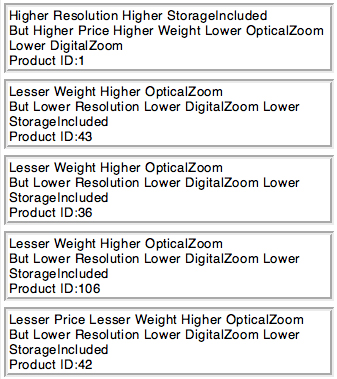
\includegraphics[width=1\linewidth]{figures-bharath/diversity1.jpg}
  \caption{Before diversifying critique strings}
  \label{fig:beforeDiv}
\end{minipage}%
\;\;\;\;\;\;
\begin{minipage}{.45\textwidth}
  \centering
  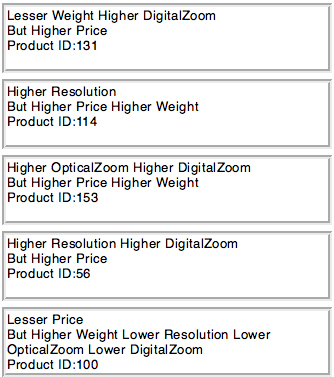
\includegraphics[width=1\linewidth]{figures-bharath/diversity2.jpg}
  \caption{After diversification}
  \label{fig:afterDiv}
\end{minipage}
\end{figure}

